\PassOptionsToPackage{table}{xcolor}

\documentclass[a4,11pt]{aleph-notas-alpha}

%%--> Paquetes adicionales
\usepackage{enumitem}
\usepackage{textcomp}
\usepackage{multicol}

%%--> Preámbulo del material
%% --> Paquetes comunes
\usepackage{listings}
\usepackage{enumitem}
\usepackage{lipsum}
\usepackage{booktabs}
\usepackage{todonotes}
\usepackage[spanish,onelanguage,vlined,linesnumbered]{algorithm2e}
\setuptodonotes{color=colordef!40, size=\footnotesize}
\newcommand{\porhacer}[1]{\todo[inline]{\textbf{Por hacer:} #1}}

%% --> Definición de colores
\definecolor{codegreen}{HTML}{A5BE00}
\definecolor{codegray}{rgb}{0.5,0.5,0.5}
\definecolor{codepurple}{rgb}{0.58,0,0.82}
\definecolor{backcolour}{rgb}{0.95,0.95,0.92}

%% --> Estilo para código
\lstdefinestyle{mystyle}{
    language={[LaTeX]TeX}, % lenguaje
    basicstyle=\bfseries\ttfamily,
    keywordstyle=\color{colordef},
    commentstyle=\color{codegreen},
    inputencoding=utf8,
    showstringspaces=false,
    flexiblecolumns=true,
    stringstyle=\ttfamily\color{blue},
    extendedchars=true,
    emph={rm,bf,it,sf}, %...
    literate=%
    {ó}{{\'o}}1%
    {í}{{\'i}}1%
    {á}{{\'a}}1%
    {ú}{{\'u}}1%
}

%% --> Selección de estilo para el código
\lstset{
    style=mystyle,escapeinside={(*@}{@*)}
}

% Blancos tipográficos
\newcommand{\mq}{\hspace{0.5em}}  %medio cuadratín
\newcommand{\tq}{\hspace{0.33em}} % un terio de cuadratín
\newcommand{\qq}{\hspace{0.25em}} % un cuarto de cuadratín
\newcommand{\fs}{\hspace{0.125em}} % un octavo de cuadratín
\newcommand{\ep}{\hspace{0.05em}} % espacio de pelo

%% --> Nota para el material
\newcommand{\informacion}{\noindent{\small\color{colordef}
El presente material fue desarrollado por:

\begin{center}
\textbf{Daniel Lara}\\
\emph{Facultad de Ciencias, Escuela Politécnica Nacional}\\[2mm]


\textbf{Andrés Merino}\\
\emph{Facultad de Ciencias Exactas y Naturales, Pontificia Universidad Católica del Ecuador}
\end{center}

\medskip\noindent
La versión actual del material es 1.3-(Noviembre 2021). En caso de encontrar inconsistencias o errores en el presente material se pueden comunicar a \href{mailto:daniel.lara@alephsub0.org}{daniel.lara@alephsub0.org}. Para más información puedes visitar nuestro sitio web: \href{https://alephsub0.org}{alephsub0.org}. Si deseas colaborar con el desarrollo de este material, el código fuente está disponible en:   
\url{https://github.com/alephsub0/LaTeX_Guias.git}. Cualquier aporte (\emph{Pull request}) será de gran ayuda para mejorar este material. 

\medskip\noindent

\includegraphics[height=10pt]{Imagenes/CreativeCommos/cc.xlarge.png}

\includegraphics[height=10pt]{Imagenes/CreativeCommos/by.xlarge.png}

\includegraphics[height=10pt]{Imagenes/CreativeCommos/nc.xlarge.png}
Esta obra se encuentra bajo licencia Atribución-NoComercial-CompartirIgual 4.0 Internacional (CC BY-NC-SA 4.0) Para más información puede visitar: \url{https://creativecommons.org/licenses/by-nc-sa/4.0/}


%% -- > Aquí se incluyen los nombres de los colaboradores de estas guías:
% \medskip\noindent
% Otros colaboradores: Katheryn Yánes
}}

%%--> Formato para títulos
\titleformat{name=\section,numberless}[display]
  {\vspace*{-2mm}\bfseries\scshape\centering}
    {}{1ex}
    {\color{colortext}\large\titlerule\vspace{.05ex}
     }
    [\color{colortext}\vspace{.2ex}\titlerule]

\titleformat{\subsubsection}
    {\color{colortext}\normalsize\bfseries}
    {\thesubsubsection}{1em}{}
    
%% --> Datos de las guias
\universidad{Curso de \LaTeX}
\autor{Proyecto Alephsub0}
\materia{Introducción a \LaTeX}

%% --> Logos de las guias
\logouno[4.5cm]{Imagenes/Logos/LogoAlephsub0-02.png}
\longtitulo{0.6\linewidth}
\fecha{Noviembre de 2021}

%% --> Nuevos ambientes
% \definecolor{coloryt}{rgb}{0.769,0.188,0.169}
%% Ambientes
\makeatletter
%%  Keys temporales: |colorlat|
\def\tcb@@colorlat{colordef!50!black}
    \tcbset{ colorlat/.code = {\def\tcb@@colorlat{#1} } }
%%  Estilo de YouTube
\tcbset{ postitbeta/.style ={
    % -> Opciones generales
    breakable,enhanced,
    before skip=2mm,after skip=3mm,
    colback=\tcb@@color!50,colframe=\tcb@@color!20!black,
    boxrule=0.4pt,
    drop fuzzy shadow,
    left=6mm,right=2mm,top=0.5mm,bottom=0.5mm,
    sharp corners,rounded corners=southeast,arc is angular,arc=3mm,
    parbox=false,
    underlay unbroken and last = {%
        \path[fill=tcbcolback!80!black]
        ([yshift=3mm]interior.south east) --++ (-0.4,-0.1) --++ (0.1,-0.2);
        \path[draw=tcbcolframe,shorten <=-0.05mm,shorten >=-0.05mm]
        ([yshift=3mm]interior.south east) --++ (-0.4,-0.1) --++ (0.1,-0.2);
        \path[fill=\tcb@@colorlat,draw=none]
        (interior.south west) rectangle node[white]{\tcb@@icono} ([xshift=5.5mm]interior.north west);
        },
    underlay = {%
        \path[fill=\tcb@@colorlat,draw=none]
        (interior.south west) rectangle node[white]{\tcb@@icono} ([xshift=5.5mm]interior.north west);
        }
    }
    }
\makeatother

%% Recuadro para enlaces de YouTube
\definecolor{coloryt}{HTML}{ffcccc}
\newtcolorbox{tcbyoutube}
    {icono=\faYoutubePlay,color=coloryt,colorlat=red,postitbeta,colframe=red,leftright skip=1cm}
    
%% Comando para enlaces de YouTube
\newcommand{\YouTube}[4]%
    {
        \begin{tcbyoutube}
            \parbox{0.30\linewidth}{\href{#2}{\includegraphics[width=\linewidth]{#3}}}
            \hspace{2mm}
            \parbox{0.65\linewidth}{\footnotesize
            \textbf{#1}\\[1mm]
            \faLink\ \url{#2}\\[2mm]
            \scriptsize
            #4}
        \end{tcbyoutube}
    }
    
%% Recuadro para enlaces
\definecolor{coloren}{HTML}{B9F2BC}
\newtcolorbox{tcbenlace}
    {icono=\faLink,color=coloren,postit,leftright skip=1cm,fontupper=\small}

%% Recuadro para impresión
\definecolor{colorimp}{HTML}{F8F8FF}
\newtcolorbox{tcbimprimir}
    {icono=\faPrint,color=colorimp,postit,leftright skip=1cm,fontupper=\small}

%% Ambiente para código
\definecolor{colcod}{RGB}{174,218,255}
\newtcolorbox{tcbcodigo}
    {icono=\faCode,color=colcod,postit,top=-2mm,bottom=-2mm,leftright skip=1cm,fontupper=\small}

%% Ambiente para código LaTeX  
\usepackage{minted}
\usemintedstyle{borland}
\tcbuselibrary{minted}
\tcbset{listing engine=minted}
\newtcblisting{tcbLaTeX}{%
    icono=\faCode,color=colcod,postit,top=0mm,bottom=0mm,
    leftright skip=1cm,fontupper=\small,
    minted language=latex,minted style=colorful,
    listing only}
% \newtcolorbox{tcbcodigo}
%     {icono=\faCode,color=colcod,postit,top=-2mm,bottom=-2mm,leftright skip=1cm,fontupper=\small}

%% Ambiente para figuras 
\newtcolorbox[blend into=figures]{figura}[2][]
    {float=h,capture=hbox,title={#2},every float=\centering,
    arc=0mm,left=2mm,right=2mm,
    boxrule=0pt,
    colback=colordef!10,
    colbacktitle=colordef!80,fonttitle=\small,
    enhanced,attach boxed title to bottom,center title,
    #1}

%% Ambiente para tablas 
\newtcolorbox[blend into=tables]{tabla}[2][]
    {float=h,capture=hbox,title={#2},every float=\centering,
    arc=0mm,left=2mm,right=2mm,
    boxrule=0pt,
    colback=colordef!10,
    colbacktitle=colordef!80,fonttitle=\small,
    enhanced,center title,
    #1}

%% Ambiente para código LaTeX desplegado
\newtcblisting{tcbLaTeXb}{%
    icono=\faCode,color=colcod,postit,top=0mm,bottom=0mm,
    fontupper=\small,
    minted language=latex,minted style=colorful,listing side text}
\newtcblisting{tcbLaTeXs}{%
    icono=\faCode,color=colcod,postit,top=0mm,bottom=0mm,
    fontupper=\small,
    minted language=latex,minted style=colorful}

%% Recuadro para comando en línea
\DeclareTotalTCBox{\miverb}{ v }{
    fontupper=\ttfamily,nobeforeafter,tcbox raise base,arc=0pt,outer arc=0pt,
    top=0pt,bottom=0pt,left=0mm,right=0mm,
    leftrule=0pt,rightrule=0pt,toprule=0.3mm,bottomrule=0.3mm,boxsep=0.5mm,
    colback=colcod!10!white,colframe=colcod!50!black}{#1}


% -- Datos del libro
\nota{Guía 1}
\tema{Primeros pasos}
%%--> Opciones adicionales
\DontPrintSemicolon

%%%%%%%%%%%%%%%%%%%%%%%%%%%%%%%%%%%%%%%%
%%  Comienzo del documento
%%%%%%%%%%%%%%%%%%%%%%%%%%%%%%%%%%%%%%%%

\begin{document}

\encabezado

\informacion

\tableofcontents

\newpage
\vspace*{-18mm}
%%%%%%%%%%%%%%%%%%%%%%%%%%%%%%%%%%%%%%%%
\section{La filosofía de \LaTeX}
%%%%%%%%%%%%%%%%%%%%%%%%%%%%%%%%%%%%%%%%

El proceso para la generación profesional de un documento escrito se lo puede dividir en tres etapas:
\begin{itemize}
\item 
    Escritura: es cuando el \textit{autor} plasma sus ideas concentrándose únicamente es el fondo del documento más no en su forma (formato), entregando un manuscrito.
\item
    Maquetación: es cuando el \textit{maquetador} decide el formato del documento (tamaño de página, márgenes, número de columnas, tipografía, espaciado, etc.), entregando una lista de instrucciones a seguir.
\item
    Composición: es cuando el \textit{compositor} usa el manuscrito del autor y la lista de instrucciones del maquetador para generar el documento final a ser publicado.
\end{itemize}
Con esto en mente, el autor debe \textit{concentrarse únicamente en escribir}, pues es el maquetador, quien con su experticia en la diagramación de textos, decide el formato adecuado. 

Dado que, no siempre contamos con el equipo necesario (maquetadores y compositores) para la generación de un documento escrito profesional, varios gestores de texto (como \textit{Microsoft Word}) generaron entornos para cargar todo este trabajo al autor, proporcionando un sistema que lo que se ve en pantalla es lo que se obtiene como resultado. Esto coloca una carga extra sobre los autores que ahora deben lidiar con el formato del documento en lugar de \textit{enfocarse en escribir}.

Para salvarnos de esto, Donald Knuth y Leslie Lamport (ambos matemáticos) nos regalaron, respectivamente, las siguientes herramientas: \TeX{} y \LaTeX{}. Antes de ver qué son estas herramientas, podemos decir, a muy breves rasgos, qué hacen:
\begin{itemize}
\item 
    \LaTeX{} es un maquetador de documentos, y
\item
    \TeX{} es un compositor de documentos.
\end{itemize}
Así, si nos ayudamos de estas herramientas, como autores, podemos dedicarnos a nuestra labor, es decir \textit{dedicarnos solo a escribir}.

Por otro lado, siempre es necesario tener cierta comunicación con nuestro maquetador, por ejemplo, decirle qué partes de nuestro texto son títulos o que partes son una lista numerada; esto lo podemos realizar colocando \textit{marcas} dentro de nuestro texto y dado que no queremos perder atención mientras vamos escribiendo, lo mejor sería que estas marcas también estén de forma escrita, por ejemplo:
\begin{tcbcodigo}\begin{lstlisting}
(esto es un título de sección) Filosofía de LaTeX (aquí termina el título)

El proceso para la generación...   
\end{lstlisting}\end{tcbcodigo} 

Ahora, dado que nuestro maquetador será un sistema informático, será necesario que estas marcas sean estandarizadas de tal forma que \LaTeX{} siempre las entienda, por esta razón, \LaTeX{} cuenta con toda una serie de \textit{marcas espaciales}, que se denominan comandos, haciendo que el ejemplo anterior quede de la siguiente manera:
\begin{tcbLaTeX}
\section{Filosofía de LaTeX}

El proceso para la generación...
\end{tcbLaTeX}
Al conjunto de comando se lo conoce como \textit{lenguaje \LaTeX{}} o \textit{código \LaTeX{}}, por lo tanto, podemos decir que \LaTeX{} es un \textit{lenguaje de marcado}.

Una vez que hemos terminado de escribir nuestro texto, colocando algunas marcas para darle indicaciones a \LaTeX{}, es necesario realizar un proceso para que nuestro maquetador interprete nuestras marcas y, junto con nuestro compositor, genere el documento final. A este proceso se lo denomina \textit{compilación} es realizado por un \textit{compilador}. El principal compilador del lenguaje \LaTeX{} se llama, de igual forma, compilador \LaTeX{}, aunque existen otro como pdf\LaTeX. Al realizar este proceso con el código del ejemplo anterior, obtenemos nuestro resultado final: el inicio de esta sección.

Como acabamos de ver, al referirnos a \LaTeX{}, podemos estar haciendo mención a varias cosas, pero todas ellas encaminadas a un mismo propósito: \textit{que el autor se concentre solo en escribir su documento}, de todo lo demás se encarga \LaTeX{}.


%%%%%%%%%%%%%%%%%%%%%%%%%%%%%%%%%%%%%%%%
\section{¿Qué necesitamos?}
%%%%%%%%%%%%%%%%%%%%%%%%%%%%%%%%%%%%%%%%

En primer lugar, dado que solo debemos concentrarnos en escribir nuestro documento y colocar las marcas adecuadas para que \LaTeX{} haga todo lo demás, necesitamos únicamente un editor de texto plano, de este tipo hay muchos: Bloc de notas, TextEdit, Gedit; sin embargo, dado que vamos a escribir código, es recomendable utilizar un editor especializado para \LaTeX{} o que tenga complementos para código \LaTeX{}. Algunas opciones son: \TeX Maker, Kile, WinEdt o Visual Studio Code; pero como se mencionó, basta con un simple Bloc de notas.

Por otro lado, necesitamos todos los programas necesarios para generar la compilación, aunque podríamos instalarlos uno por uno, es mejor instalar todo en conjunto. Para esto, existen las \textit{distribuciones de \LaTeX{}} que nos instalan todos los programas necesarios\footnote{Algunas distribuciones vienen también con editores de texto especializados para \LaTeX.}; algunas de estas distribuciones son: MiK\TeX, Mac\TeX, \TeX{}Live.

Una vez que tengamos esto, podemos escribir en las siguientes líneas las siguientes líneas en un archivo y llamarlo, por ejemplo, \texttt{MiPrimerArchivo.tex}:
\begin{tcbLaTeX}
\documentclass[11pt]{article}

\begin{document}
    Hola Mundo
\end{document}
\end{tcbLaTeX}


Notemos que la \textit{extensión} del archivo es \texttt{.tex}, con esto indicaremos a \LaTeX{} que este es un archivo donde está el manuscrito que realizamos, es decir, todo archivo que quiera compilarlo con \LaTeX{} debe tener extensión \texttt{.tex}.

Ahora, para pedir a \LaTeX{} que realice todo el trabajo para generar nuestro documento final, debemos realizar la compilación del archivo \texttt{MiPrimerArchivo.tex}. Esto lo podemos lograr abriendo un \textit{terminal} de nuestro computador en la misma carpeta que tenemos nuestro archivo\footnote{En Windows, esto se consigue abriendo el explorador de archivos en la carpeta que tengamos nuestro archivo y escribiendo en la barra de direcciones el texto: \texttt{cmd} y dando un enter} y escribir:
\begin{tcbcodigo}\begin{lstlisting}
    pdflatex MiPrimerArchivo.tex
\end{lstlisting}\end{tcbcodigo}
Así, pedimos que se compile nuestro archivo utilizando el compilador pdf\LaTeX{}.
Podemos ver esto en la Figura~\ref{fig:001}, ejecutamos este comando (damos enter) y \LaTeX{} se pondrá manos a la obra y nos devolverá nuestro primer archivo PDF generado utilizando \LaTeX{}.

\begin{figura}[label={fig:001}]
    {Captura de la ventana de comandos ejecutando \LaTeX{} en Windows.}
    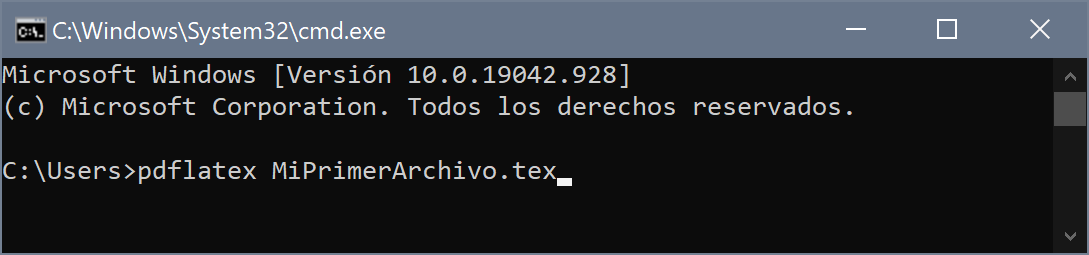
\includegraphics[width=0.75\textwidth]{Imagenes/guia01-1.png}
\end{figura}


\subsection{¿Todo esto para dos palabras?}

Sí, pero con dos indicaciones: primero, los editores especializados tiene <<botones>> especializados para que hagan todo el proceso de compilación con un solo clic; segundo, es el mismo proceso tanto para nuestro archivo de dos palabras como para un libro de cientos de páginas. Además, ya conocemos brevemente la secuencia de trabajo con \LaTeX{}:
\begin{enumerate}
    \item Escribir nuestro documento.
    \item Compilar nuestro documento.
\end{enumerate}

Una consideración adicional, si deseamos obviar todo esto de la instalación, podemos usar servicios en la nube los cuales ya tienen instalado las distribuciones necesarias y nos presentan un editor de texto especializado para escribir código \LaTeX{}, la más popular de todas (y en la cual basaremos estas guías) es \textit{Overleaf}, en la cual solo necesitamos crearnos una cuenta y ya podremos iniciar a escribir nuestros documentos. Aquí, podemos dividir nuestro trabajo en \textit{proyectos} e ingresando a cada proyecto ya podremos escribir nuestro texto y compilarlo; podemos ver la interfaz de Overleaf en la Figura~\ref{fig:002}.


\begin{figura}[label={fig:002}]
    {Interfaz de nuestros documentos en Overleaf.}
    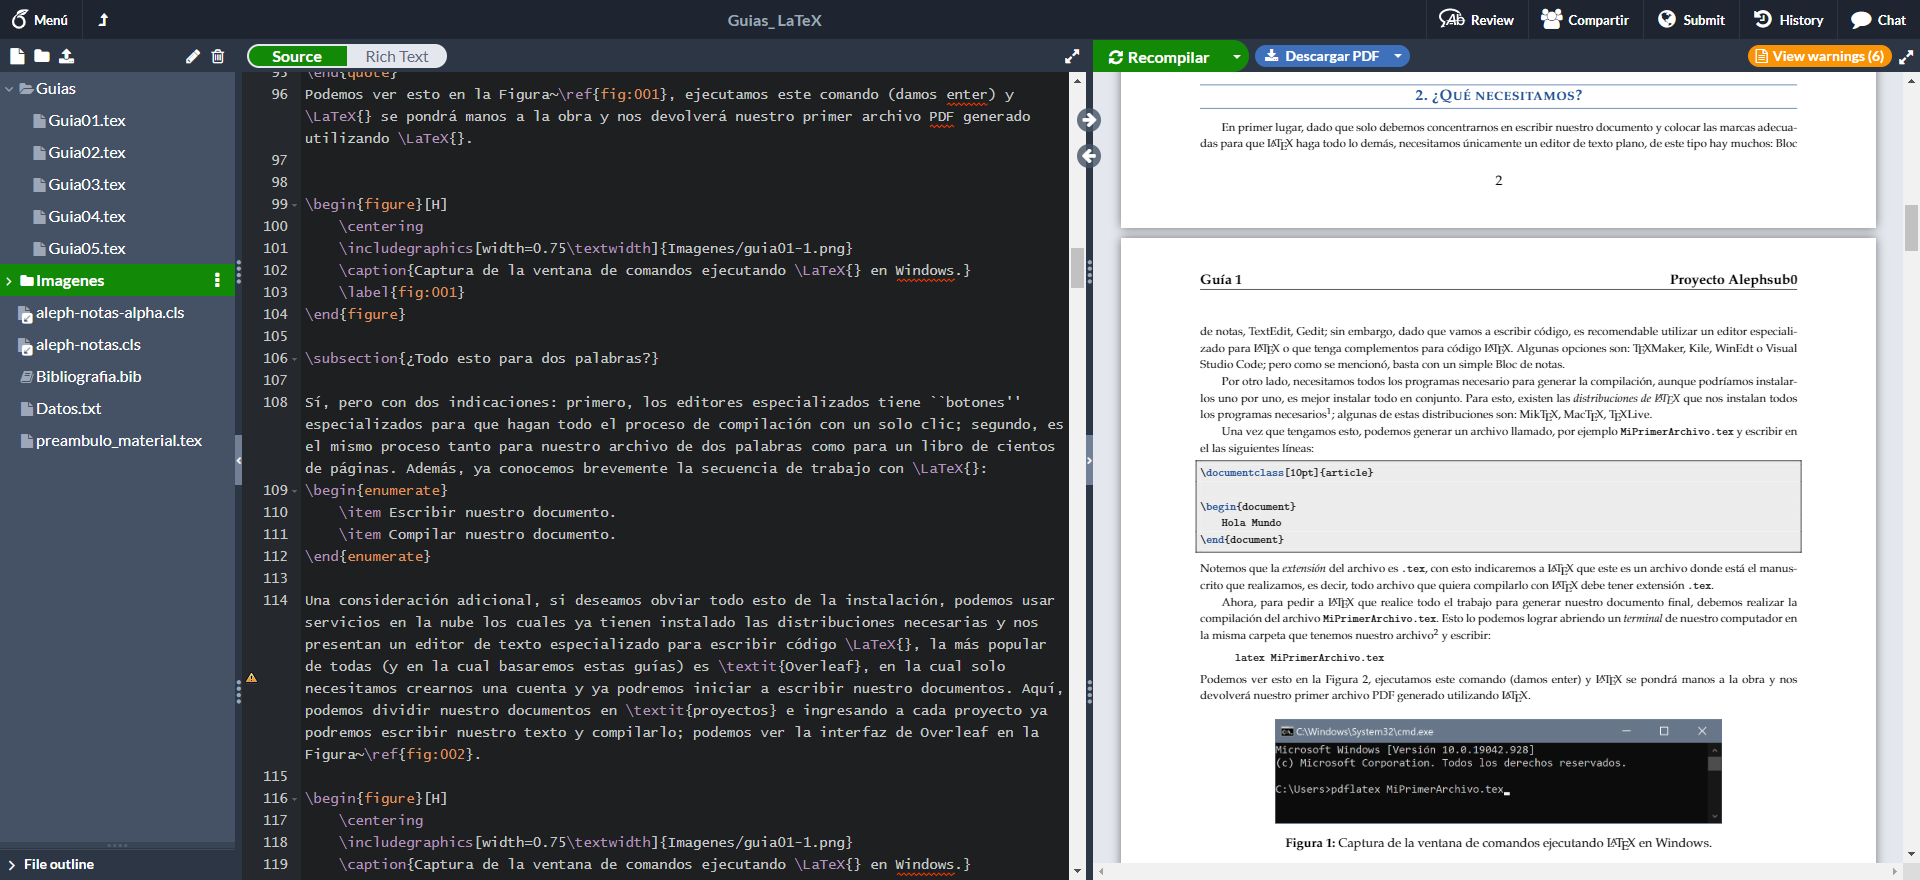
\includegraphics[width=0.95\textwidth]{Imagenes/guia01-2.png}
\end{figura}


%%%%%%%%%%%%%%%%%%%%%%%%%%%%%%%%%%%%%%%%
\section{Antes de iniciar}
%%%%%%%%%%%%%%%%%%%%%%%%%%%%%%%%%%%%%%%%

\subsection{Consideraciones sobre el editor}

Al trabajar con \LaTeX{}, casi la totalidad del tiempo estaremos escribiendo código. Por esta razón para que nuestro trabajo sea eficiente es necesario tener adecuadamente configurado nuestro teclado, un video sobre este tema se puede encontrar en el siguiente enlace:
\YouTube{¿Cómo configurar cualquier teclado para escribir en español?}
    {https://link.alephsub0.org/ConfiguracionTeclado}
    {Imagenes/Portada18.png}
    {Te enseñamos cómo configurar de manera correcta cualquier teclado, esté en español o inglés, para utilizarlo al escribir en español, además, te indicamos cómo usarlo luego de configurado.}


Por otro lado, podemos aprovechar las ventajas de los atajos de teclado de nuestro editor y de esta forma realizar un uso casi exclusivo del teclado para el desarrollo de nuestro trabajo. Los principales atajos de teclado del editor de Overleaf son:
\begin{multicols}{2}\small
\begin{itemize}
    \item \verb"Ctrl + enter" para compilar.
    \item \verb"Ctrl + /" para comentar el código.
    \item \verb@Ctrl + Home@ mueve al inicio del documento.
    \item \verb@Ctrl + End@ mueve al final del documento.
    \item \verb@Ctrl + L@ mueve a la línea especificada.
    \item \verb@Ctrl + D@ elimina la línea actual.
    \item \verb@Ctrl + B@ texto en negrita.
    \item \verb@Ctrl + I@ texto en itálica.
    \item \verb"Ctrl + F" para buscar y reemplazar.
    \item \verb"Shift + Tab" para eliminar sangría.
\end{itemize}
\end{multicols}

\begin{tcbenlace}
    Una lista completa se puede encontrar en:\\ 
    \faLink\ \url{https://es.overleaf.com/learn/how-to/Hotkeys}
\end{tcbenlace}


\subsection{Consideraciones sobre la redacción}

Al momento de redactar un texto, debemos tener en cuenta la siguiente premisa: Todo dentro de un texto o es un párrafo, o es parte de un párrafo, o es un título, o es un flotante (imagen, tabla, etc.). Dado que, en general, lo que predomina en un texto son párrafos, asumiremos que, a menos que se indique lo contrario, todo lo que escribimos es un párrafo o parte de uno.


\subsection{Algunos sitios de utilidad}

Antes de comenzar el trabajo en \LaTeX{} es importante tomar en cuenta los siguientes enlaces para los recursos que nos serán de utilidad a lo largo del curso:

\begin{itemize}[leftmargin=*]\small
    \item
        Página de Overleaf: \url{https://www.overleaf.com/}
    \item
        Página oficial de \TeX Maker: \url{https://www.xm1math.net/texmaker/}
   \item
        Página oficial de MiK\TeX: \url{http://miktex.org/}
   \item
        Red de completa de archivos \TeX: \url{http://www.ctan.org/}
   \item 
        Catálogo en línea de paquetes de \LaTeX: \url{http://www.ctan.org/pkg/_A}
   \item
        Grupo de usuarios \TeX: \url{http://www.tug.org/}
    \item
        Comunidad de usuarios \LaTeX{} de Stack Exchange: \url{https://tex.stackexchange.com/}
\end{itemize}


%%%%%%%%%%%%%%%%%%%%%%%%%%%%%%%%%%%%%%%%
\section{Generalidades}
%%%%%%%%%%%%%%%%%%%%%%%%%%%%%%%%%%%%%%%%

Regresemos a nuestro archivo \texttt{MiPrimerArchivo.tex}:
\begin{tcbLaTeX}
\documentclass[11pt]{article}

\begin{document}
    Hola Mundo
\end{document}
\end{tcbLaTeX}
En la primera línea de este archivo, podemos notar el comando \miverb{\documentclass[11pt]{article}}; en general esta es la sintaxis básica de todo comando de \LaTeX{}:
\begin{itemize}
\item 
    Todo comando de \LaTeX{} inicia con la barra inversa <<\miverb"\">>.
\item
    Luego de la barra inversa, sin espacio, va el nombre del comando (en este caso, el nombre del comando es \miverb{documentclass}).
\item
    A continuación, entre corchetes, se coloca los argumentos opcionales; como su nombre lo indica, estos argumentos podría no ser necesarios, en cuyo caso, simplemente se elimina esta parte quedando: \miverb{\documentclass{article}}.
\item   
    Finalmente, entre llaves, se coloca los argumentos obligatorios; existen comandos que no requieren ningún argumento obligatorio, en esos casos, el comando solo cuenta con la barra inversa y el nombre del comando.
\end{itemize}

En nuestro caso, nuestro comando \miverb{\documentclass[11pt]{article}} sirve para definir el formato general del documento, algunas posibilidades disponibles para el argumento obligatorio son 
\begin{multicols}{4}
\begin{itemize}
    \item \miverb@article@;
    \item \miverb@report@;
    \item \miverb@book@;
    \item \miverb@slides@;
    \item \miverb@beamer@;
    \item \miverb@letter@;
    \item \miverb@standalone@;
    \item \miverb@minimal@.
\end{itemize}
\end{multicols}
Cada una de estas definirá el formato general del documento como la geometría de la página, el formato para encabezados, títulos, etc. Por otra parte, el argumento opcional \miverb{10pt} define el tamaño de fundición (tamaño de letra), otras posibilidades para este argumento son:
\begin{multicols}{3}
\begin{itemize}
    \item \miverb@10pt@;
    \item \miverb@11pt@;
    \item \miverb@12pt@.
\end{itemize}
\end{multicols}
Este argumento es opcional dado que, si no lo colocamos, tomará el valor por defecto que, en el caso de \miverb{article}, es de \miverb{10pt}, es decir, colocar
\begin{tcbLaTeX}
\documentclass[10pt]{article}
\end{tcbLaTeX}
\noindent
es equivalente a colocar
\begin{tcbLaTeX}
\documentclass{article}
\end{tcbLaTeX}


El siguiente comando que observamos en nuestro archivo es \miverb"\begin{document}", este marca el inicio del \textbf{cuerpo del documento}, todo lo que se coloque antes de este comando, se lo denomina \textbf{preámbulo del documento}. Finalmente, tenemos el comando \miverb"\end{document}", el cual marca el final del cuerpo del documento.

Todo archivo debe tener, como mínimo, estos tres comandos; el primer comando que aparezca en el documento siempre debe ser \miverb"\documentclass" y todo lo que esté luego del comando \miverb"\end{document}" será ignorado en la compilación.

\begin{advertencia}
    Para compilar un documento exitosamente se requiere que siempre exista contenido entre \miverb"\begin{document}" y \miverb"\end{document}". Si intentamos compilar un documento con esta sección vacía, este proceso se detendrá sin resultado alguno.
\end{advertencia}

El comando \miverb"\begin" tiene un carácter especial pues define lo que se conoce como \textbf{ambientes}, por lo cual, siempre que se coloque un comando \miverb"\begin", debe estar emparejado con un comando \miverb"\end" para que se delimite el alcance del ambiente. Por ejemplo, para utilizar un ambiente ficticio llamado \texttt{foo}, se debe utilizar el siguiente esquema:
\begin{tcbLaTeX}
Texto fuera del ambiente foo.
\begin{foo}
    Texto dentro del ambiente foo.
\end{foo}
Texto fuera del ambiente foo.
\end{tcbLaTeX}
\noindent
En los párrafos anteriores, utilizamos el ambiente \miverb{document} para escribir todo el contenido de nuestro documento.

%%%%%%%%%%%%%%%%%%%%%%%%%%%%%%%%%%%%%%%%
\section{Paquetes}
%%%%%%%%%%%%%%%%%%%%%%%%%%%%%%%%%%%%%%%%

\LaTeX{} cuenta con una abundante cantidad de comandos y ambientes que podemos utilizar para escribir nuestro documento, por ejemplo, el comando \miverb"\today", el cual imprime la fecha en la que se compila el documento. Veamos el siguiente ejemplo, el código:
\begin{tcbLaTeX}
\documentclass[11pt]{article}

\begin{document}
    La fecha en que se escribió este documento es \today.
\end{document}
\end{tcbLaTeX}
\noindent genera el siguiente texto:
\begin{tcbimprimir}
    La fecha en que se escribió este documento es  \foreignlanguage[date]{english}{\today}.
\end{tcbimprimir}

Como podemos apreciar, se imprimió lo que esperábamos, pero en inglés, ya que es el idioma por defecto en el que trabaja \LaTeX{} y no le indicamos que íbamos a escribir en español. Para esto, necesitamos introducir lo que se conoce como \textbf{paquetes}.

Un \textbf{paquete de \LaTeX{}} es un archivo que incluye comandos destinados a agregar nuevas funciones o redefinir funciones ya existente o facilitar su uso.

\begin{tcbenlace}
    La lista oficial de paquetes disponibles, junto con su documentación, se pueden encontrar en:\\ 
    \faLink\ \url{https://ctan.org/}{https://ctan.org/}
\end{tcbenlace}

Para incluir un paquete se debe utilizar la siguiente sintaxis, siempre en el preámbulo del documento:

\begin{tcbLaTeX}
\usepackage[Opciones del paquete]{Nombre del paquete}
\end{tcbLaTeX}

Para escribir textos en español, los paquetes básicos que se debe utilizar son los siguientes:
\begin{itemize}
    \item
        \miverb{babel}: Gestiona el idioma del documento, en nuestro caso, utilizaremos la opción \miverb{spanish}.
    \item 
        \miverb{inputenc}: Gestiona la codificación de caracteres\footnote{Ver más: \url{https://es.wikipedia.org/wiki/Codificacion_de_caracteres}} de entrada, esto nos permitirá escribir directamente desde nuestro teclado los caracteres especiales del español (por ejemplo las tildes). La opción para el paquete depende del editor que estemos utilizando, en nuestro caso, al utilizar Overleaf, colocaremos la opción \miverb{utf8}.
    \item
        \miverb{fontenc}: Gestiona la codificación de caracteres de salida, esto nos permitirá que, al momento de tener nuestro documento PDF y copiar texto de él, los caracteres especiales sean reconocidos correctamente. La opción que utilizaremos es \miverb{T1}.
\end{itemize}

Con los paquetes mencionados es posible comenzar la composición de un documento, quedando nuestro ejemplo de la siguiente manera:
\begin{tcbLaTeX}
\documentclass[10pt]{article}

\usepackage[utf8]{inputenc}
\usepackage[T1]{fontenc}
\usepackage[spanish]{babel}

\begin{document}
    La fecha en que se escribió este documento es \today.
\end{document}
\end{tcbLaTeX}
\noindent genera el siguiente texto:
\begin{tcbimprimir}
    La fecha en que se escribió este documento es \today.
\end{tcbimprimir}

Conforme avancemos en los contenidos, introduciremos nuevos paquetes que ampliarán las herramientas que disponemos. No obstante, para el desarrollo de un documento, se recomienda trabajar únicamente con los paquetes requeridos para evitar conflictos en la compilación del documento.

\subsection{El paquete \texttt{babel}}

Como mencionamos anteriormente, el paquete \miverb{babel} gestiona el idioma del documento, con esto, nos referimos a que adapta la estructura del documento a las particularidades propias del idioma. Algunas de estas particularidades son:
\begin{itemize}
\item 
    Nombres de los elementos del documento: por ejemplo, los títulos de resúmenes, tablas de contenidos o la misma fecha que vimos anteriormente, entre otros.
\item
    Separación en sílabas de las palabras para cortes al final de cada línea.
\item
    Formato de los párrafos, formato de números romanos, formato de separador decimal, formato de listas, formato de sangría.
\end{itemize}

El paquete \miverb{babel} admite alrededor de 50 idiomas diferentes y dentro de cada idioma tiene varias opciones para configurar detalles especiales. Por ejemplo, para el idioma español el experto en ortotipografía\footnote{Conjunto de normas para el uso correcto de la tipografía.} Javier Bezos planteó y programó las opciones que pueden ser utilizadas por el paquete \miverb{babel}.

\begin{tcbenlace}
    La lista de opciones para el idioma español del paquete \miverb{babel} puede ser consultada en:\\ 
    \faLink\ \url{http://www.texnia.com/spanishopt.html}\\
    Las bases para estas opciones pueden ser consultadas en:\\
    \faLink\ \url{http://www.texnia.com/spanish2.html}    
\end{tcbenlace}


\subsection{El paquete \texttt{geometry}}

Otro paquete importante, pero no fundamental, es el paquete \miverb{geometry}, el cual nos ayuda con una de las primeras tareas a realizar en la preparación de un documento: definir su tamaño, márgenes y otras medidas.

Por ejemplo, si deseamos cambiar el tamaño de hoja a un tamaño A5, en orientación horizontal y con 2~cm de margen a cada lado, basta colocar las siguientes opciones al incluir el paquete:

\begin{tcbLaTeX}
\usepackage[a5paper, landscape, margin=2cm]{geometry}
\end{tcbLaTeX}

En cuanto a tamaño de hoja, existen varios argumentos que pueden ser utilizados, los más comunes pueden ser los de la serie A de la ISO para utilizarlos, estos están descritos en el Cuadro~\ref{tab:dimensioneshojas}. También se puede definir el tamaño de hoja de forma personalizada mediante los argumentos \miverb{paperwidth}, \miverb{paperheight} o \miverb{papersize} de la siguiente manera:
\begin{tcbLaTeX}
\usepackage[papersize = {10cm, 20cm}]{geometry}
\end{tcbLaTeX}
\noindent
o, de forma equivalente:
\begin{tcbLaTeX}
\usepackage[paperwidth = 10cm , paperheight = 20cm]{geometry}
\end{tcbLaTeX}


\begin{tabla}[label = {tab:dimensioneshojas}]
    {Algunos tamaños de hojas disponibles}
    \rowcolors{2}{colordef!17}{colordef!10}
    \begin{tabular}{ccc}
    \toprule
    \textbf{Argumento} &  \textbf{Normativa } &  \textbf{Dimensiones} \\ \midrule
    \verb"a0paper" & ISO - DIN Serie A0 & 841mm $\times$ 1189mm \\
    \verb"a1paper" & ISO - DIN Serie A1 & 594mm $\times$ 841mm \\
    \verb"a2paper" & ISO - DIN Serie A2 & 420mm $\times$ 594mm \\
    \verb"a3paper" & ISO - DIN Serie A3 & 297mm $\times$ 420mm  \\
    \verb"a4paper" & ISO - DIN Serie A4 & 210mm $\times$ 297mm \\
    \verb"a5paper" & ISO - DIN Serie A5 & 148mm $\times$ 210mm 
    \\\bottomrule
    \end{tabular}
\end{tabla}

En lo que respecta a orientación de la hoja, para horizontal se utiliza el argumento \miverb{landscape} y para vertical, \miverb{portrait}; sin embargo, esta última es la opción por defecto, por lo tanto, podría omitirse. Finalmente, para los márgenes, existen varias formas de definirlas; si queremos tener las mismas medidas en todos los márgenes podemos colocar
\begin{tcbLaTeX}
\usepackage[margin = 4cm]{geometry}
\end{tcbLaTeX}
\noindent
si queremos dar una misma medida a los márgenes verticales (arriba y abajo) y hacer lo propio con los horizontales (izquierda y derecha), podemos colocar
\begin{tcbLaTeX}
\usepackage[vmargin = 2cm, hmargin = 3cm]{geometry}
\end{tcbLaTeX}
\noindent
por último, si queremos dar medidas diferentes a cada margen, colocamos
\begin{tcbLaTeX}
\usepackage[right = 2cm, left = 1cm, top = 3cm, bottom = 4cm]{geometry}
\end{tcbLaTeX}
\noindent
o, de manera equivalente\footnote{Notemos que realizar un salto de línea entre las opciones no ocasiona ningún inconveniente y mejora la visualización del código.},
\begin{tcbLaTeX}
\usepackage[rmargin = 2cm, lmargin = 1cm, 
            tmargin = 3cm, bmargin = 4cm]{geometry}
\end{tcbLaTeX}

El paquete \miverb{geometry} dispone de muchas más opciones para controlar varios otros aspectos de la geometría de la hoja y se puede consultar en su documentación.

\begin{tcbenlace}
    La documentación del paquete \miverb{geometry} puede ser consultada aquí:\\ 
    \faLink\ \url{https://ctan.org/pkg/geometry}    
\end{tcbenlace}


Con lo aprendido hasta ahora, tenemos que la estructura base de cualquiera de nuestros documentos puede verse algo así:
\begin{tcbLaTeX}
\documentclass[11pt]{article}

\usepackage[utf8]{inputenc}
\usepackage[T1]{fontenc}
\usepackage[spanish]{babel}

\usepackage[a4paper, margin = 3cm]{geometry}

\begin{document}
    Mi primer documento en \LaTeX.
\end{document}
\end{tcbLaTeX}

\end{document} 